% mnras_guide.tex
%
% MNRAS LaTeX user guide
%
% v3.1 released 11 June 2020
%
% v3.0 released 22 May 2015
% (version numbers match those of mnras.cls)
%
% Copyright (C) Royal Astronomical Society 2015
% Authors:
% Keith T. Smith (Royal Astronomical Society)

% Change log
%
% v3.0   September 2013 - May 2015
%    First version: complete rewrite of the user guide
%    Basic structure taken from mnras_template.tex by the same author

%%%%%%%%%%%%%%%%%%%%%%%%%%%%%%%%%%%%%%%%%%%%%%%%%%
% Basic setup. Most papers should leave these options alone.
\documentclass[fleqn,usenatbib,useAMS]{mnras}

%%%%% AUTHORS - PLACE YOUR OWN PACKAGES HERE %%%%%

% Only include extra packages if you really need them. Common packages are:
\usepackage{graphicx}	% Including figure files
\usepackage{amsmath}	% Advanced maths commands
\usepackage{amssymb}	% Extra maths symbols
\usepackage{multicol}        % Multi-column entries in tables
\usepackage{bm}		% Bold maths symbols, including upright Greek
\usepackage{pdflscape}	% Landscape pages

%%%%%%%%%%%%%%%%%%%%%%%%%%%%%%%%%%%%%%%%%%%%%%%%%%

%%%%%% AUTHORS - PLACE YOUR OWN MACROS HERE %%%%%%

% Please keep new commands to a minimum, and use \newcommand not \def to avoid
% overwriting existing commands. Example:
%\newcommand{\pcm}{\,cm$^{-2}$}	% per cm-squared
\newcommand{\kms}{\,km\,s$^{-1}$} % kilometres per second
\newcommand{\bibtex}{\textsc{Bib}\!\TeX} % bibtex. Not quite the correct typesetting, but close enough

%%%%%%%%%%%%%%%%%%%%%%%%%%%%%%%%%%%%%%%%%%%%%%%%%%


% Use vector fonts, so it zooms properly in on-screen viewing software
% Don't change these lines unless you know what you are doing
\usepackage[T1]{fontenc}
\usepackage{ae,aecompl}

% MNRAS is set in Times font. If you don't have this installed (most LaTeX
% installations will be fine) or prefer the old Computer Modern fonts, comment
% out the following line
\usepackage{newtxtext,newtxmath}
% Depending on your LaTeX fonts installation, you might get better results with one of these:
%\usepackage{mathptmx}
%\usepackage{txfonts}

%%%%%%%%%%%%%%%%%%% TITLE PAGE %%%%%%%%%%%%%%%%%%%

% Title of the paper, and the short title which is used in the headers.
% Keep the title short and informative.
	\title[Kalman PTA]{State-space PTA}

% The list of authors, and the short list which is used in the headers.
% If you need two or more lines of authors, add an extra line using \newauthor
\author[Kimpson]{Kimpson$^{1}$, Melatos,O'Leary, , Evans, others, etc. %
\thanks{Contact e-mail: \href{mailto:mn@ras.ac.uk}{mn@ras.ac.uk}}%
\thanks{Present address: Science magazine, AAAS Science International, \mbox{82-88}~Hills Road, Cambridge CB2~1LQ, UK}%
\\
% List of institutions
$^{1}$Royal Astronomical Society, Burlington House, Piccadilly, London W1J 0BQ, UK}

% These dates will be filled out by the publisher
\date{Last updated 2020 June 10; in original form 2013 September 5}

% Enter the current year, for the copyright statements etc.
\pubyear{2020}

% Don't change these lines
\begin{document}
\label{firstpage}
\pagerange{\pageref{firstpage}--\pageref{lastpage}}
\maketitle

% Abstract of the paper
\begin{abstract}
This is an abstract
\end{abstract}

% Select between one and six entries from the list of approved keywords.
% Don't make up new ones.
\begin{keywords}
editorials, notices -- miscellaneous
\end{keywords}

%%%%%%%%%%%%%%%%%%%%%%%%%%%%%%%%%%%%%%%%%%%%%%%%%%

%%%%%%%%%%%%%%%%% BODY OF PAPER %%%%%%%%%%%%%%%%%%

% The MNRAS class isn't designed to include a table of contents, but for this document one is useful.
% I therefore have to do some kludging to make it work without masses of blank space.
\begingroup
\let\clearpage\relax
%\tableofcontents
\endgroup
\newpage

\section{Introduction}



The detection of high frequency ($\sim 1$Hz) gravitational waves (GWs) from coalescing BH binaries with ground-based detectors such as LIGO/Virgo \citep{aLIGO,2015CQGra..32b4001A} is now a routine enterprise \citep[e.g.][]{2019PhRvX...9c1040A,2021PhRvX..11b1053A}. Gravitational radiation from sources which radiate in the mill-Hz regime are expected to be detectable from $\sim 2030$ with the space-based Laser Interferometer Space Antenna, \citep{LISApaper} especially given the early success by the pathfinder mission \citep{2019arXiv190308924A}. Detecting GWs from systems which evolve over even longer timescales, $\mathcal{O}$(years), has necessitated the development of novel astrophysical methods, since it is practically impossible to engineer interferometric detectors with sufficiently long baselines. The foremost technique for the detection of GWs in this nano-Hz regime is a via timing an ensemble of milliseconds pulsars; a pulsar timing array (PTA) \citep{2021hgwa.bookE...4V}. The presence  of a nano-Hz gravitational wave will influence the propagation of the pulsar radio beacon, leaving a characteristic impression on the pulsar timing signal. By measuring the modulation of the received pulsar signal in this way, one can effectively construct a detector with a baseline on the scale of parsecs. \newline 


\noindent Multiple PTA detectors have now been built over the last few decades, including the North American Nanohertz Observatory for Gravitational Waves \citep[NANOGrav,][]{2020ApJ...905L..34A}, the Parkes Pulsar Timing array \citep[PPTA][]{2020PASA...37...20K}, and the European Pulsar Timing Array \citep[EPTA,][]{2010CQGra..27h4014F}. These previously disparate efforts have now been joined in international collaboration, along with a number of newer PTAs, under the umbrella of the International Pulsar Timing Array \citep[IPTA][]{2019MNRAS.490.4666P}. The primary target of PTA observations is the gravitational radiation emitted from the inspiral of supermassive black hole binaries (SMBHBs) with masses $\sim\mathcal{ 10^7 M_{\odot}}$. These GW signals from SMBHBs can be broadly classified into either deterministic or stochastic. For the former, sufficiently bright and near binaries may be resolvable with PTAs, allowing the very earliest stages of their evolution and coalescence to be investigated. For the latter, the incoherent superposition of multiple weaker SMBHBs sources leads to a stochastic background detectable at nano-Hz frequencies. Other potential sources for PTAs include cosmic strings \citep[e.g.][]{PTAstring} and cosmological phase transitions \citep[e.g.][]{PTAphase}, but the deterministic and stochastic GW signals from SMBHBs remain the primary targets. \newline 



\noindent The detection of loud, resolved sources with a PTA typically involves a parametrised model for the pulsar timing residuals induced by the modulation of the pulsar signal by a GW. One can then search for evidence that this model describes the data via the usual Bayesian likelihood techniques, and try to estimate the parameters of the model \citep[e.g.][]{Babak2016}. For detecting the stochastic background the approach is different; one measures the correlation in pulsar timing residuals between any two pair of pulsars. The presence of a GW induces a characteristic correlation function as a function of the angular separation between the pulsars; the Hellings-Downs curve \citep{Hellings}. For both classes of source, detection of GW signals in the timing residuals of a PTA is a challenging enterprise, and currently neither a stochastic background nor an individually resolved source has yet been detected \citep{2022MNRAS.510.4873A, 10.1093/nsr/nwx126}. \newline 


\noindent Motivated by the difficulties faced by the classic PTA analysis methods, in this work we present a novel approach to formulate PTA analysis and GW detection as a state-space problem. This approach enables the state-space evolution to be tracked optimally, and for a specific realisation of the pulsar process noise (i.e. the spin wandering of the pulsar) infer both the system parameters and the detectability of the GW signal. For this initial exploratory study we will focus exclusively on resolved, monochromatic GW sources. 




This paper is organised as follows.


\footnote{1. Introduce PTAs generally. 2.Types of astrophysical source to be detected with PTAs. 3. Previous methods. 4. Challenges/problems of previous methods. 5. Our approach and its potential advantages. }




\section{State-Space Model}
We want to formulate the PTA analysis as a state-space problem with a separation between the intrinsic pulsar state and the measurement state recorded by an observer. We will take our state to be the pulsar pulse frequency $f(t)$. We will now consider how the intrinsic pulse frequency evolves in time, completely separate from the influence of a GW, and then go on to derive the  influence of a GW perturbation on the frequency recorded by an observer at Earth.

\subsection{Evolution of the pulsar frequency}
We will take as our model of the intrinsic pulsar frequency $f$ a variation of the phenomenological model of \citep{Vargas}. Within this model, $f$ evolves according to a combination of both deterministic torques (i.e. electromagnetic spin-down) and stochastic torques (i.e. `spin wandering', achromatic variations in the pulse TOA intrinsic to the star). The deterministic torque is taken to arise from the pulsar magnetic dipole, with braking index $n=3$ whilst the stochastic torque is a simple white noise process. Specifically, the frequency evolves according to a Ornstein-Uhlenbeck process (equivalently a Langevin equation) with a time-dependent drift parameter:
\begin{equation}
	\frac{df}{dt} = -\gamma	 [f - f_{\rm EM} (t)] + \dot{f}_{\rm EM} + \xi(t)
	\label{eq:frequency_evolution}
\end{equation}
where $f_{\rm EM}$ is the solution of the electromagnetic spindown equation, $\gamma$ a proportionality constant, and $\xi(t)$ a white noise process that satisfies,
\begin{equation}
	\langle \xi(t) \xi(t') \rangle = \sigma^2 \delta(t - t')
\end{equation}
For PTA analysis, we are concerned with timescales on the order of years. Consequently, we can express the EM spindown straightforwardly as
\begin{equation}
	f_{\rm EM} (t) = f_{\rm EM}(0) + \dot{f}_{\rm EM} (0)t
\end{equation}  
Completely, the frequency evolution is then given by the solution of the stochastic differential equation,
\begin{equation}
	\frac{df}{dt} = -\gamma	 [f - f_{\rm EM}(0) - \dot{f}_{\rm EM} (0)t] + \dot{f}_{\rm EM} (0) + \xi(t)
	\label{eq:frequency_evolution_expanded}
\end{equation}
As emphasised in \cite{Vargas}, this model for the frequency evolution is a phenomenological model that aims to qualitatively reproduce the typical behaviour of observed pulsars, rather than being derived from a physical model of the neutron star \citep[e.g. a model of the neutron star crust and superfluid components][]{Meyers2021}. However, for our purposes of exploring the detection of GWs via a state space formulation it will prove sufficiently accurate and appropriate.

\subsection{Modulation of pulsar frequency due to a GW}
In the presence of a GW, the $f(t)$ measured by an observer on Earth is different from that measured by an observer in the local NS reference frame. We want to determine how the GW influences the received frequency

\subsubsection{Plane GW perturbation}
We take a gravitational plane wave that perturbs a background Minkowski spacetime as
\begin{equation}
	g_{\mu \nu} = \eta_{\mu \nu} + H_{\mu \nu} e^{i(\Omega(\bar{n} \cdot \bar{x} - t) + \Phi_0)	}
\end{equation}
for spatial coordinates $\bar{x}$, where the GW has a constant angular frequency $\Omega$, propagates in the $\bar{n}$-direction and has a phase offset of  $\Phi_0$. We emphasise that $\Omega$ has no time dependence - we are concerned solely with monochromatic sources. Note that we are free to choose our coordinate system such that $\Phi_0$ is the GW phase at $t=0$ \textit{at the Earth.}\footnote{\textbf{TK: This point is important, since the phase offset is then the same between multiple pulsars. See also Melatos 2022 PT12}}. The amplitude tensor $H_{\mu \nu}$ has zero temporal components ($H_{0 \mu} = H_{\mu 0} = 0$) whilst the spatial part is
\begin{align}
	H_{ij} = h_+ e_{ij}^+(\bar{n}) + h_{\times} e_{ij}^{\times}(\bar{n})
\end{align}
where  $h_{+,\times}$ are the polarisation amplitudes of the gravitational plane wave. The polarisation tensors $e_{ij}^{+,\times}$ are uniquely defined by the principal axes of the wave:
\begin{equation}
	e_{a b}^{+}(\hat{\Omega}) =\hat{m}_a \hat{m}_b-\hat{n}_a \hat{n}_b
\end{equation}
\begin{equation}
		e_{a b}^{\times}(\hat{\Omega}) =\hat{m}_a \hat{n}_b+\hat{n}_a \hat{m}_b
\end{equation}
which are in turn specified via the location of the GW source on the sky (via $\theta$, $\phi$ coordinates) and the polarisation angle $\psi$
\begin{align}
	\vec{m} & =(\sin \phi \cos \psi-\sin \psi \cos \phi \cos \theta) \hat{x} \nonumber \\
	& -(\cos \phi \cos \psi+\sin \psi \sin \phi \cos \theta) \hat{y} \nonumber \\
	& +(\sin \psi \sin \theta) \hat{z} \\
	\vec{n} & =(-\sin \phi \sin \psi-\cos \psi \cos \phi \cos \theta) \hat{x} \nonumber \\
	& +(\cos \phi \sin \psi-\cos \psi \sin \phi \cos \theta) \hat{y}\nonumber  \\
	& +(\cos \psi \sin \theta) \hat{z}
\end{align}

\subsubsection{Pulse frequency as a photon}
\noindent We will consider the pulse frequency as a photon with covariant 4-momentum $p_{\mu}$. Generally, the frequency of a photon recorded by an observer with 4-velocity $u^{\mu}$ is 
\begin{equation}
	\nu = p_{\alpha} u^{\alpha}
\end{equation}
\noindent We consider both our emitter and receiver to be stationary, such that  
\begin{equation}
	u^{\alpha}|_{\rm emitter} = u^{\alpha}|_{\rm receiver} = (1,0,0,0)
\end{equation}
\noindent Consequently the frequency can be directly identified with the temporal component of the covariant 4-momentum,
\begin{equation}
	f = p_t
\end{equation}
\noindent The expression for the evolution of the pulse frequency as measured by the observer on Earth is then,
\begin{equation}
	p_t(t_1)|_{\rm Earth} = p_t(t_0)|_{\rm source} + \int_{t = t_0}^{t=t_1} \dot{p}_t dt
\end{equation}
\noindent where the overdot denotes a derivative w.r.t. $t$. Since the influence of the GW perturbation on $\dot{p}_t$ is small, we can relate the source emission and receiver times as $t_1 = t_0 + d$ and consider the photon trajectory to be an unperturbed path. \footnote{\textbf{TK: See also e.g. Maggiore, Meltaos who takes the same approach...}} \newline 

\noindent To complete our expression, we now just need to determine $\dot{p}_t$ and integrate it.

\subsubsection{Hamiltonian Mechanics}
The Hamiltonian in covariant notation can be written as 
\begin{equation}
	H(x^{\mu}, p_{\mu}) = \frac{1}{2} g_{\mu \nu} p^{\mu} p^{\nu},
\end{equation}
\noindent which if we substitute in our expression for the perturbed metric is
\begin{equation}
	H = \frac{1}{2} \eta_{\mu \nu} p^{\mu} p^{\nu} + \frac{1}{2} H_{ij}p^i p^j e^{i(\Omega(\bar{n} \cdot \bar{x} - t) + \Phi_0)	}
\end{equation}
\noindent Now, Hamilton's equations are
\begin{equation}
	\frac{dx^{\mu}}{d\lambda} = \frac{\partial H}{\partial p_{\mu}} , \, \, \frac{dp_{\mu}}{d \lambda} = -\frac{\partial H}{\partial x^{\mu}} 
\end{equation}

\noindent for affine parameter $\lambda$. The derivative of the temporal component of the covariant momenta is then,
\begin{equation}
	\frac{d p_{t}}{d \lambda} = -\frac{i\Omega}{2} H_{ij}p^i p^j  e^{i(\Omega(\bar{n}\cdot \bar{x} - t))+\Phi_0}
\end{equation}
\footnote{\textbf{TK: This is equivalent to Melatos 2018, Eq 5 for the specific case of a GW propagating in the $z$-direction, with zero phase offset}.}


\noindent Therefore the derivative w.r.t coordinate time $t$ is,
\begin{equation}
	\dot{p}_t = \frac{d p_{t}}{d \lambda} \left(\frac{dt}{d\lambda}\right)^{-1} = \frac{d p_{t}}{d \lambda} \left(\frac{1}{p^t}\right)
\end{equation}
\noindent Note that $\dot{p}_t$ is entirely a function of the GW perturbation. In the Minkowski case the spacetime is stationary and so $p_t$ should be conserved along the geodesic. It will prove useful to recognise that $p^{\mu} = \omega(1,-q^x,-q^y,-q^z)$ where $\bar{q}$ is the unit vector between the Earth and pulsar and $\omega$ is the \textit{constant} photon angular frequency. Given the small effect of the GW perturbation, at first order we can identify $\omega$ as either the frequency at source or observer \footnote{see Melatos 2022, PT16}. We will consider  the pulsar locations to be constant with respect to the Earth. TK: \textbf{This may have already been "done" during the barycentreing when pulsar TOAs are generated, in which case $q$ is the vector from the SSB to the pulsar}. Similarly we can express the spatial coordinates as $\bar{x}(t) = -\bar{q}t$. \newline  


\noindent Bringing this all together we can write $\dot{p}_t$ in a condensed form as,
\begin{equation}
	\dot{p}_t = A e^{i \gamma t + \Phi_0}
\end{equation}
where 
\begin{equation}
	\gamma = -\Omega (1 + \bar{n}\cdot \bar{q}) 
\end{equation}
\footnote{compare with Melatos 2022, PT11}
\noindent and
\begin{equation}
	A = -\frac{i\Omega \omega}{2} H_{ij}q^i q^j 
\end{equation}

\subsubsection{Performing the integral}

The frequency shift experienced by the observer relative to the source due to a GW is then
\begin{align}
	p_t(\tau)|_{\rm Earth} - p_t(\tau - d)|_{\rm source} = A \int_{t = \tau - d}^{t=\tau} e^{i \gamma t + \Phi_0}dt  \\
	=\frac{-iA}{\gamma} e^{i \gamma \tau}e^{\Phi_0}[1 - e^{-i \gamma d}] 
	\label{eq:concise}
\end{align}
We can write this more explicitly as,
\begin{align} \label{eq:final}
	&p_t(\tau)|_{\rm Earth} - p_t(\tau - d)|_{\rm source} = \\
	&\frac{ \omega}{2} \frac{H_{ij}q^i q^j  }{(1 + \hat{n} \cdot \hat{q})}e^{-i \Omega \tau(1+\bar{n} \cdot \bar{q}) + \Phi_0} [1 - e^{i \Omega(1+\bar{n} \cdot \bar{q}) d}]
\end{align}
or alternatively, with $h_{ij} = g_{ij} - \eta_{ij}$,
\begin{equation}
	p_t(\tau)|_{\rm Earth} - p_t(\tau - d)|_{\rm source} =\frac{ \omega}{2} \frac{h_{ij} q^i q^j  }{(1 + \hat{n} \cdot \hat{q})} [1 - e^{i \Omega(1+\bar{n} \cdot \bar{q}) d}]
	\label{eq:freq_shift}
\end{equation}

\subsection{State-space structure} \label{sec3}
We now have a model for the evolution of the pulsar frequency states and the measured frequency timeseries. We can express the intrinsic frequency evolution, Eq. \ref{eq:frequency_evolution_expanded}, in a alternative form as,
\begin{equation}
	df = A f dt + N(t) dt + \sigma dB(t)
	\label{eq:state1}
\end{equation}
where $A = -\gamma$, $N(t) = \gamma(f_{\rm EM}(0) + \dot{f}_{\rm EM}(0) t) +\dot{f}_{\rm EM}(0)$ and $dB(t)$ denotes increments of Brownian motion (Wiener process). This equation is easily identified as an Ornstein-Uhlenbeck process which has a general solution given by,
\begin{equation}
	f(t) = e^{At}f(0) + \int_0^t e^{A(t-t')} N(t') dt' + \int_0^t e^{A(t-t')} \sigma dB(t')
\end{equation} 
If we move from a solution in continuous time to discrete time then
\begin{equation}
	f(t_{i+1}) = F f(t_i) + T_i + \eta_i
\end{equation}
where
\begin{equation}
	F_i = e^{A (t_{i+1} - t_i)}
\end{equation}
\begin{equation}
	T_i = \int_{t_i}^{t_{i+1}}  e^{A (t_{i+1} - t')} N(t') dt'
\end{equation}
\begin{equation}
	\eta_i = \int_{t_i}^{t_{i+1}}  e^{A (t_{i+1} - t')} \sigma dt'
\end{equation}
Given the discrete solution $f(\bar{t})$ where $\bar{t} = (t_1, t_2, ...,t_N)$ the intrinsic frequency can be related to the measured frequency as 
\begin{equation}
	f_M = f g(\bar{\theta},t) + N_M
\end{equation}
where $g(\theta,t)$ ("measurement function")is a function of some parameters, $\bar{\theta}$ and time $t$, whilst $N_M$ is a Gaussian measurement noise that satisfies 
\begin{equation}
	\langle N_M(t) N_M(t') \rangle = \Sigma^2 \delta(t - t')
\end{equation}
The measurement function follows from Eq. \ref{eq:freq_shift}
\begin{equation} \label{eq:final}
	g(\bar{\theta},t) = 1 - \frac{1}{2} \frac{h_{ij}(t) q^i q^j}{1 + \bar{n} \cdot \bar{q}}[1 - e^{i \Omega(1+\bar{n} \cdot \bar{q}) d}]
\end{equation}
or in a more concise form where we have switched to a trigonometric form of the equations,
\begin{equation} 
	g(\bar{\theta},t) = 1 -A \cos(-\Omega t (1 + n\cdot q ) + \Phi_0)
\end{equation}
where 
\begin{equation}
	A =  \frac{1}{2} \frac{H_{ij} q^i q^j}{1 + \bar{n} \cdot \bar{q}}[1 - \cos\left( {\Omega(1+\bar{n} \cdot \bar{q}) d}\right)]
		\label{eq:state2}
\end{equation}


\section{Detection and parameter estimation}
Given the proceeding state-space model we will now try to use this model to infer the unknown parameters of the system. Let's first review and categorise all the parameters of model. We can generally separate these into parameters which correspond to the intrinsic frequency evolution of the pulsar, the GW parameters and the noise parameters i.e.
\begin{equation}
	\bar{\theta} =  \bar{\theta}_{\rm PSR} \cup \bar{\theta}_{\rm GW} \cup \bar{\theta}_{\rm noise}
\end{equation}
\begin{equation}
	\bar{\theta}_{\rm PSR} = [\gamma, f_{\rm EM}(0), \dot{f}_{\rm EM}(0),d]
\end{equation}
\begin{equation}
	\bar{\theta}_{\rm GW} = [h_{+}, h_{\times}, \delta, \alpha, \psi, \Omega, \Phi_0]
\end{equation}
\begin{equation}
	\bar{\theta}_{\rm noise} = [\sigma, \Sigma]
\end{equation}
Whilst the GW parameters are shared between measurements for each pulsar, the pulsar parameters are clearly not. For a PTA dataset of N pulsars we have $7 + 5N$ parameters to estimate. For now we will consider the measurement noise to be known, although in principle this too could be estimated. Note that whilst this is a large parameter space, in general the pulsar parameters are much better constrained than the GW parameters: for example we have rough estimates for the pulsar distances accurate to $\sim$ 10$\%$, but we have no prior information on the source location. \newline 

\noindent We will use a Kalman filter in order to obtain likelihood estimates of the data given a set of parameters. We will now review the Kalman filter and the associated likelihood in Section \label{sec:kalman_filter} before going on to discuss how to use nested sampling methods in conjunction with the filter for detection (model selection) and parameter estimation

\subsection{Kalman Filtering}\label{sec:kalman_filter}
The Kalman filter \citep{Kalman1} is a algorithmic technique for recovering a set of system state variables $\bar{x}$ given some noisy measurements $\bar{z}$. It is a common technique in signal processing that has also been applied more recently with great success in astrophysics \citep[e.g.][]{Meyers2021,Melatos2023}. The linear Kalman filter operates on measurements that are related to states via a linear transformation
\begin{equation}
	z = Hx + v
\end{equation}
where $H$ is the measurement matrix and $v$ a Gaussian measurement noise. The underlying states are the solutions to the state-space equation 
\begin{equation}
	\dot{x} = Fx + Gu + w
\end{equation}
where $x$ are the state variables, $F$ the system dynamics matrix, $G u$ the control matrix/vector and $w$ a stochastic zero-mean process which .  By comparison with the preceding equations Eqs. 	\ref{eq:state1} - 	\ref{eq:state2} it is immediately obvious how our state space model maps onto the Kalman filter structure. Specifically, our states are just the $N$ intrinsic pulsar frequencies $\bar{x} = (f_1,f_2,...f_N)$ whilst our measurements are the $N$ measured pulse frequencies $\bar{z} = (f^{(M)}_1,f^{(M)}_2,...f^{(M)}_N)$. If we specialize to the case of constant time sampling between our observations, then for our formulation, the various components that make up the Kalman filter are as follows: 
\begin{equation}
	F_i = F_{i+1} = e^{-\gamma \Delta t}
\end{equation}
\begin{align}
	T_i &= \int_{t_i}^{t_{i+1}}  e^{A (t_{i+1} - t')} N(t') dt' \\
	    & =
\end{align}






The Kalman filter includes the effect of process noise and measurement noise via the defines a measurement noise matrix $R = E[v v^T]$
defines a process noise matrix $Q = E[w w^T]$.

\begin{equation}
	\eta_i = \int_{t_i}^{t_{i+1}}  e^{A (t_{i+1} - t')} \sigma dt'
\end{equation}

















Whilst for our problem we only need concern ourselves with linear stuff

%Extensions to non-linear state-transitions
%[i.e. 𝑭𝑿 → 𝑓 (𝑿) in equation (11)], and non-linear measurement
%equations [i.e. 𝑪𝑿 → 𝑐(𝑿) in equation (10)] can be achieved using a range of tools such as the extended Kalman filter (Jazwinski
%1970), the unscented Kalman filter (Julier & Uhlmann 1997; Wan
%& Merwe 2000; Julier & Uhlmann 2004), or particle filters (Del
%Moral 1997).
%The full set of Kalma
%
for a full review we refer the reader to X





the state the states are related to a measurement via

where this is that is this



By comaprison with the state space equations we derived earlier (Eqs A to B) we can see that our continuous equations map ideally onto this structure. In particular, for our system our state $\bar{x}$ is simply the frequencies of each individual pulsar $= (f_1, f_2, f_3,...)$



here is an example for an arbitary GW and arbitrary pulsar with good and bad parameters 
\subsection{Nested Sampling}

We can use NS for both param estimation and 



\section{Validation on synthetic data}








\subsection{PTA pulsars}
Throughout this work it will be necessary to select a group of pulsars to make up our PTA. We will take the 47 pulsars that make up the NANOGrav PTA \citep{2020ApJ...905L..34A}





In order to proceed and explore how well this state-space formulation works, we will need to specify a selection of pulsars to make up our PTA. We will take the 47 pulsars that make up the NANOGrav PTA. For each pulsar, we need to specify the complete set of $\bar{\theta}_{\rm PSR}$ as well as $\sigma$. The parameters $f_{\rm EM}(0), \dot{f}_{\rm EM}(0),d$ are straightforward to set and can be read directly from  the current "present day" best estimates of the pulsar frequency, derivative and distance. 


\begin{figure}
	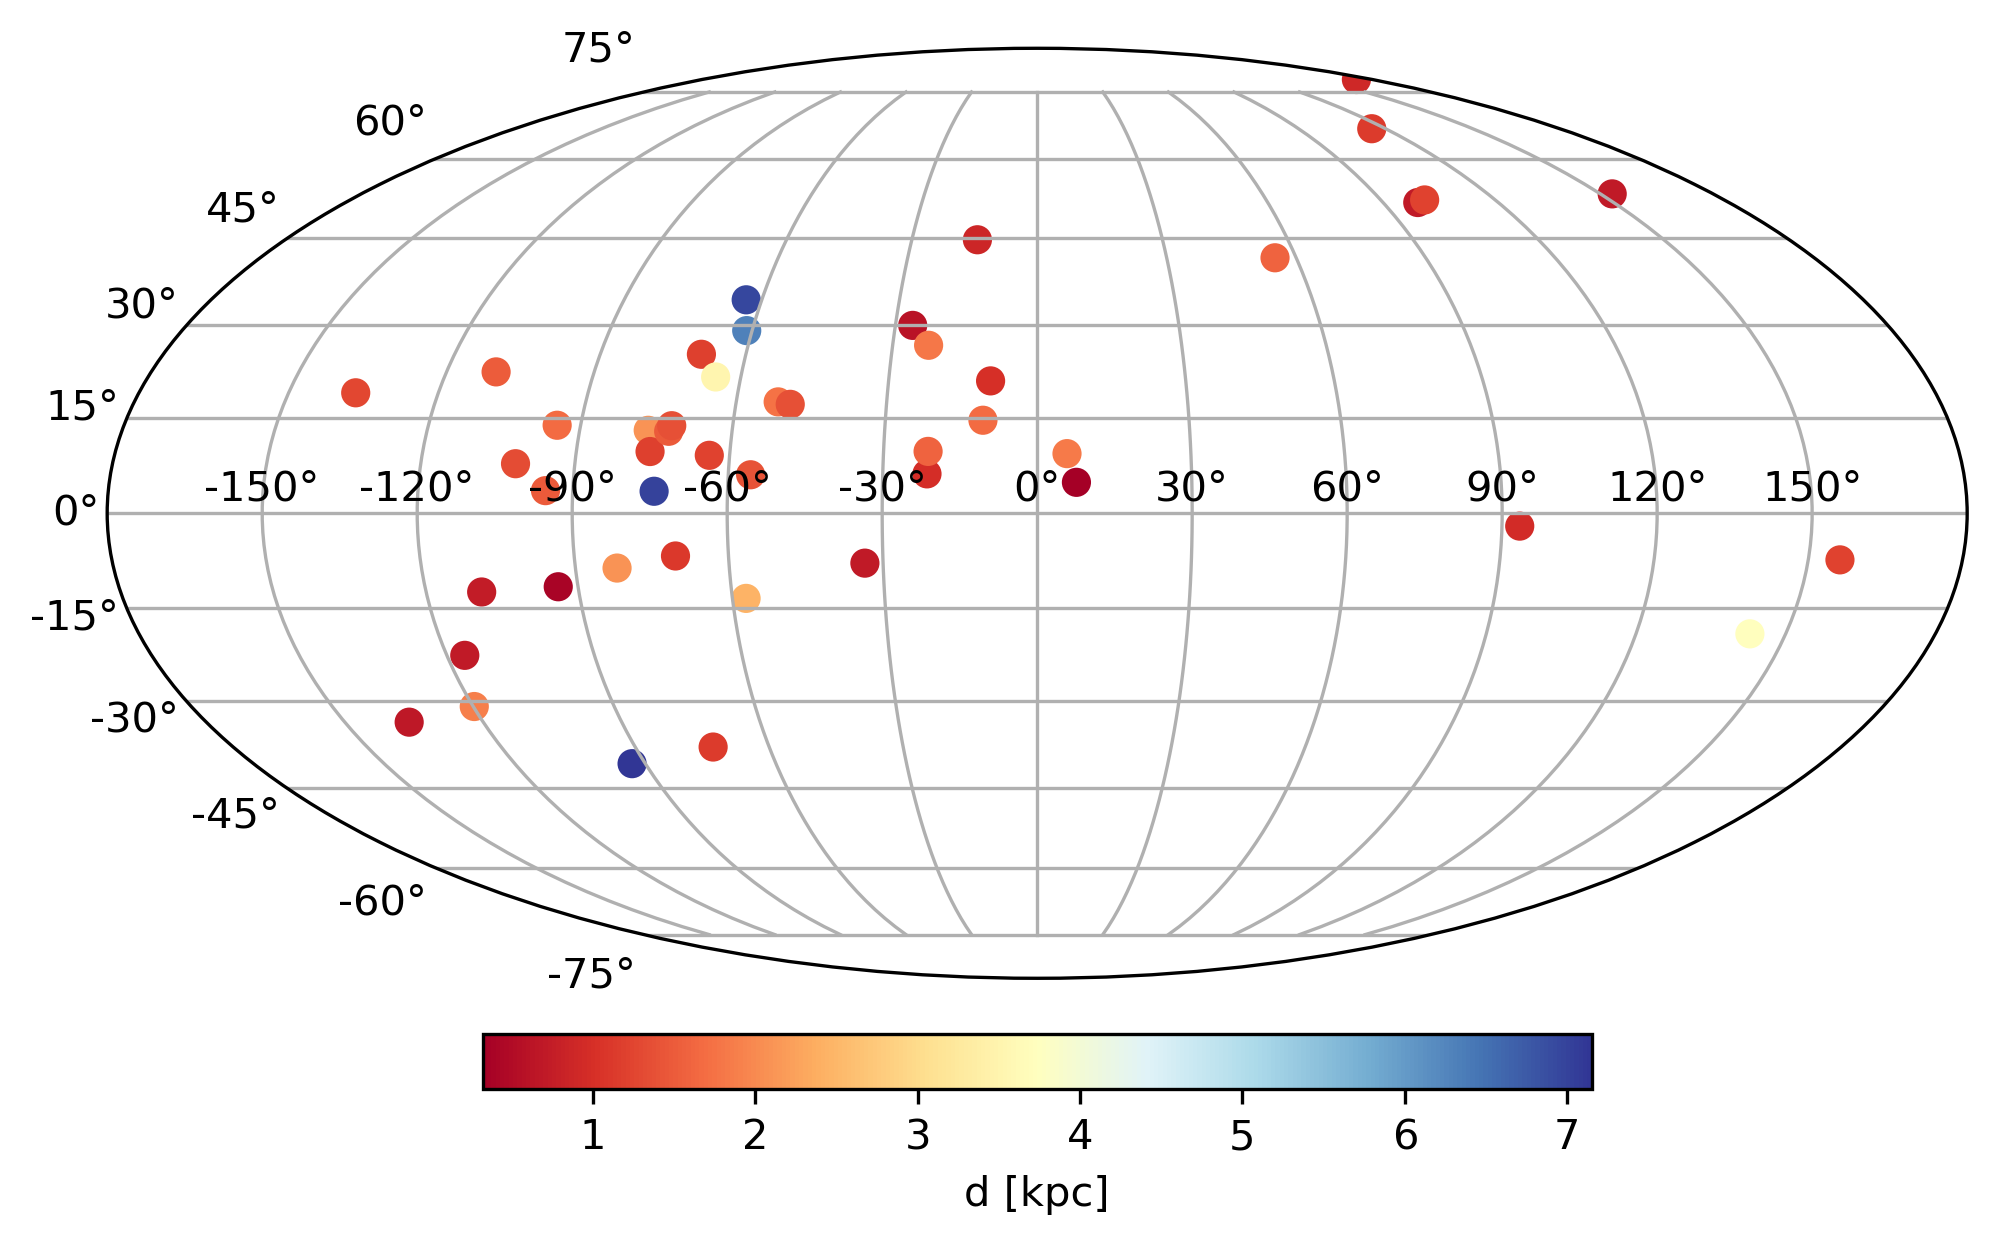
\includegraphics[width=0.8\columnwidth]{images/pulsars}
	\caption{Spatial distribution and distances of NANOGrav pulsars}
	\label{fig:pulsar_distrib}
\end{figure}


\subsection{Detection}



\subsection{Parameter Estimation}











\section{Kalman filtering}



\section{Parameter estimation}












\subsection{Nested sampling}


\section{Detection}






\noindent The general structure of a Kalman state-space problem is
\begin{equation}
	\dot{x} = f(x) + w
\end{equation}
where $x$ are the state variables, $f()$ a non-linear function of the states, and $w$ a stochastic zero-mean process. The process noise matrix $Q = E(w w^T)$. The states are related to the measurement $z$ via a non-linear measurement function $h()$
\begin{equation}
	z = h(x) + v
\end{equation}
where $v$ is a stochastic zero-mean process and measurement noise matrix $R = E(v v^T)$. \newline 


\noindent This structure maps onto the preceding equations nicely. Our hidden state is just the intrinsic pulsar frequency, which evolves as,
\begin{eqnarray}
	\dot{f}_P = -\gamma f_P^n + \xi(t)
\end{eqnarray}
where $n$ is a braking index (typical values $\sim 1-5$, we take a canonical value $=3$) \footnote{See A. Vargas talk re anomalous braking indices. P.S. is there an arXiv preprint?} $\gamma$ a proportionality constant, and $\xi(t)$ represents a stochastic white noise process. Equation \ref{eq:final} can be used to relate the intrinsic pulsar frequency to that measured by an observer on Earth:

\begin{eqnarray}
	f_M = f_p(1 - X) + N_M
\end{eqnarray}
where $X$ is the RHS of Eq. \ref{eq:final} and $N_M$ a Gaussian measurement noise. An example of the evolution of the state and the measurement frequencies for our PTA pulsars can be seen in Fig. \ref{fig:mean and std of nets}









\section{Discretisation}

This intrinsic frequency can be related to a measured frequency as 


There are a few terms to unpack and define in this equation. $q(t)$ is the vector from the Earth to the pulsar, $n$ the propagation direction of the GW, $\Omega$ the (constant) angular frequency of the GW and $d$ the Earth-pulsar distance. $h_{ij}(t)$ is the metric perturbation due to the GW $= g_{ij} - \eta_{ij}$. It is given by the familiar plane-wave relation:	
\begin{equation}
	h_{ij}(t) = H_{ij} e^{(i(\bar{k} \cdot \bar{x} - \Omega t + \Phi_0))}
\end{equation}
where $\bar{k}$ is the GW 3-wavevector $=\Omega \bar{n}$ and $x = -\bar{q} t$ (photon propagates from pulsar to Earth), and for phase offset (GW phase at Earth when $t=0$) $\Phi_0$.  We can also write this as,
\begin{equation}
h_{ij}(t) = H_{ij} e^{(-i\Omega t (1 + \bar{n} \cdot \bar{q} ) + \Phi_0))}
\end{equation}
The amplitude tensor  $H_{ij}$ is
\begin{equation}
	H_{ij} = h_+ e_{ij}^+(\bar{n},\psi) + h_{\times} e_{ij}^{\times}(\bar{n},\psi)
\end{equation}
where $h_{+,\times}$ are the constant amplitudes of the gravitational plane wave, and $e_{ij}^{+, \times}(\bar{n}, \psi)$ are the polarisation tensors which are uniquely defined by the principal axes of the GW. $\psi$ is the polarisation angle of the GW. \newline 








\noindent Going forward,  \newline 




\noindent Bringing this together, and adopting a trigonometric form of the equations, we can express the measurement equation as 






\subsection{Parameters of the model}
\noindent 



We can also express the measurement equation generally as,









Kalman filtering works as follows


you can see that it maps nicel onto our state separation 





\section{Methods}


There are two potential methods we can take

\begin{enumerate}
	\item Let the states just be the frequencies $\bar{x} = (f)$. We have a linear equation for both the state evolution and the measurement matrix. Both of these depend on the parameters $\theta$. Use the likelihood output by a standard Kalman filter to run a nested sampler and try to recover $\theta$.
	\item Let the states be the frequencies and all the unknown parameters $\bar{x} = (f, \bar{\theta}_{\rm GW},\bar{\theta}_{\rm PSR},\bar{\theta}_{\rm noise})$. Our state evolution is now linear but our measurement matrix is non-linear - a function of the states(parameters). Use a non-linear estimator such as a EKF/UKF to try to recover all of the states at once.
\end{enumerate}


\subsection{Method 1}


In the case where the states are just the intrinsic pulsar frequencies, we can write the ODEs in matrix form as
\begin{equation}
	d\bar{X} = \bar{A} \bar{X} dt + \bar{N}(t) dt + \bar{\Sigma} d\bar{B}(t) 
\end{equation}
where $\bar{A} = \text{diag}(\gamma_1, \gamma_2,...)$,  $\bar{X} = \text{diag}(f_1, f_2,...)$, $\bar{N} =\text{diag}(\gamma_1[a_1+b_1t] + b_1, ...)$
and we have let $a = f_{EM}(0)$, $b = \dot{f}_{\rm EM}(0)$.


\subsection{References}
\label{sec:ref_list}





\bibliographystyle{mnras}
\bibliography{example} % if your bibtex file is called example.bib





%%%%%%%%%%%%%%%%%%%%%%%%%%%%%%%%%%%%%%%%%%%%%%%%%%


% Don't change these lines
\bsp	% typesetting comment
\label{lastpage}
\end{document}

% End of mnras_guide.tex
